\documentclass{beamer}
\usetheme{metropolis}
\usecolortheme{seahorse}
\setbeamertemplate{frame numbering}[fraction]
\metroset{block=fill}

\usepackage[utf8]{inputenc}

\usepackage{graphicx}
\graphicspath{ {./imgs/} }

\usepackage{multicol}

\usepackage{soul} % strikethrough


\title{We Have Built Nice Things}
\subtitle{Ossification is not Stagination}
\author{Wang, Hao (she / her)}
\institute{Lead Software Architect @ Graveflex | ms-jpq @ github | hola@bigly.dog}
\date{}


\begin{document}


\begin{frame}

	\titlepage

\end{frame}


\begin{frame}{Correction}

	Wrong employer on speakers list

	\rule{\textwidth}{0.1em}

	Worked at \textit{\textbf{Sun}Cloud} not \textit{\textbf{Sound}Cloud}

\end{frame}


\begin{frame}{\$JOB}

	Software Architect @ Graveflex

	\rule{\textwidth}{0.1em}

	\begin{center}

		
\includegraphics[width=16em,height=16em]{graveflex}

	\end{center}

\end{frame}


\begin{frame}{Inspiration}

	We can have nice things - \textit{Justin M. Keyes}

	\vspace{1em}

	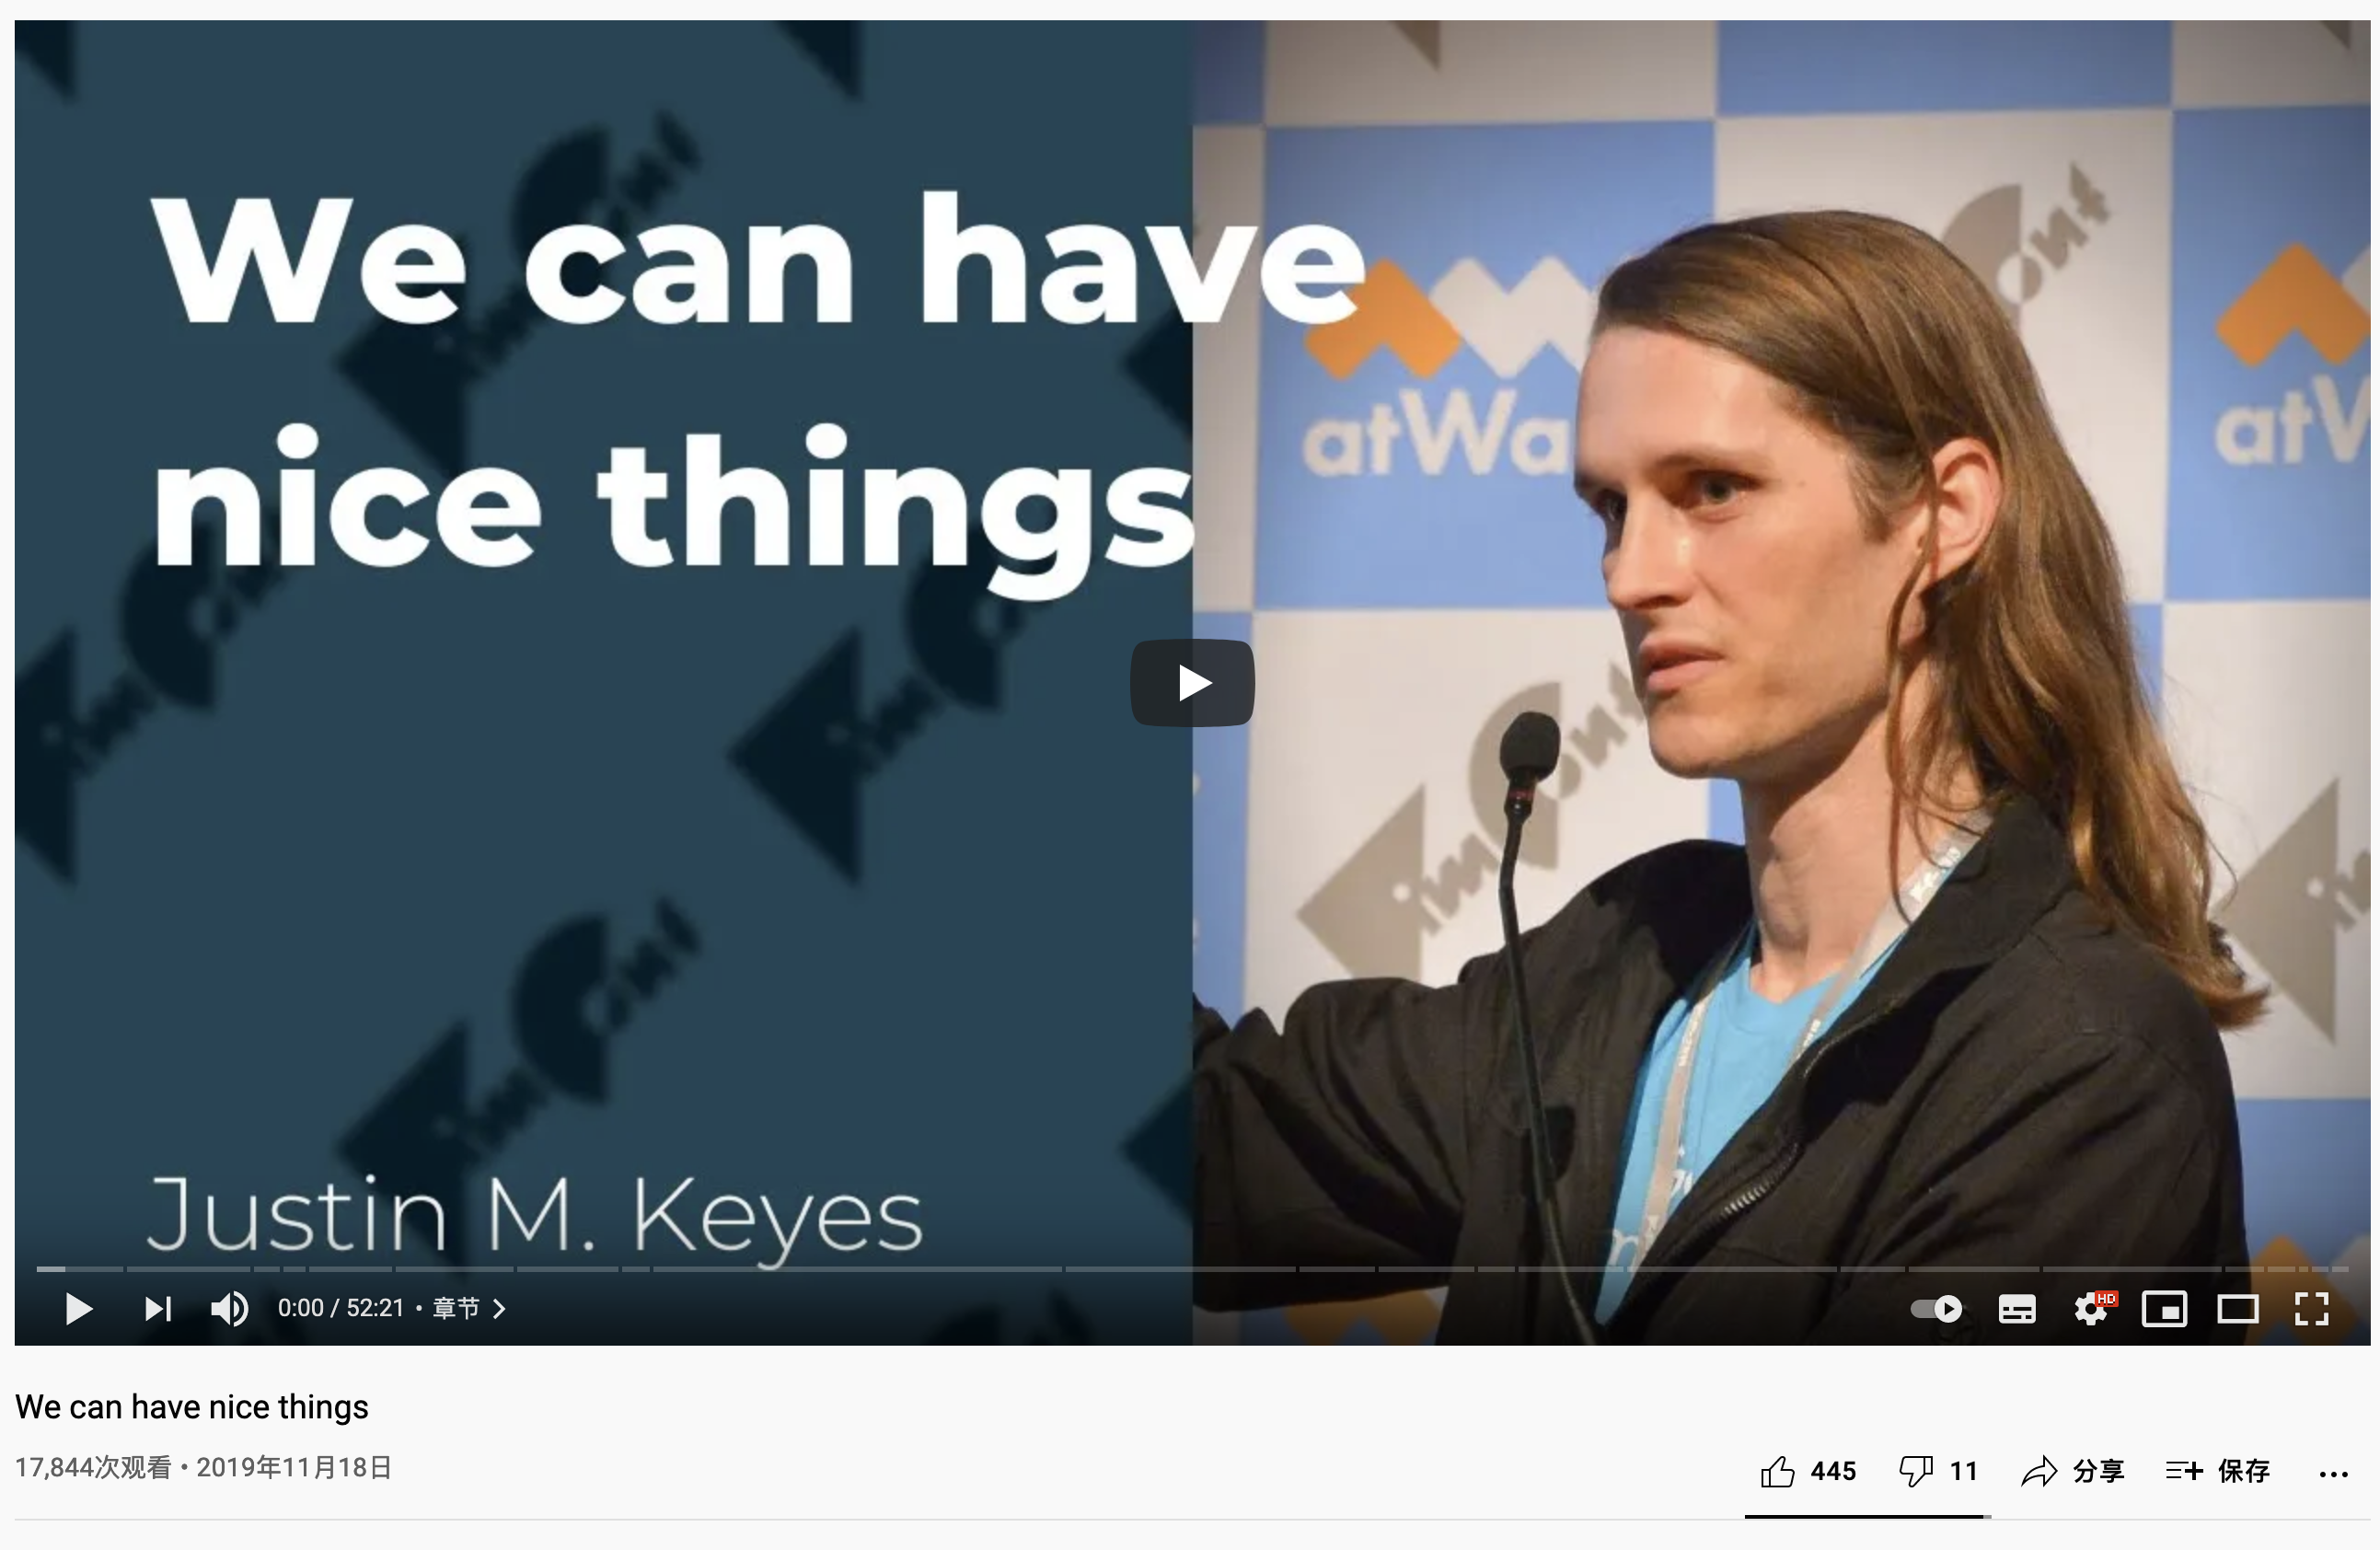
\includegraphics[width=\textwidth]{we_can_have_nice}

\end{frame}


\begin{frame}{Why Nvim?}

	I wanted to replace emacs

	\vspace{1em}

	
\includegraphics[width=\textwidth]{home_page}

	\vspace{1em}

\end{frame}


\begin{frame}{Talk}

	\textbf{Ossification} in Nvim

	\rule{\textwidth}{0.1em}

	\begin{itemize}

		\item CHADTree

		      File manager

		      \hspace{0.1em}

		\item COQ.nvim

		      Auto completion

	\end{itemize}

	\rule{\textwidth}{0.1em}

\end{frame}


\begin{frame}{Ossification -> Innovation}

	\textbf{Ossofication is not Stagnation}

	\rule{\textwidth}{0.1em}

	\begin{itemize}

		\item Nvim has comes with a historied legacy

		\item Consequences of legacy

		\item Gifts of legacy

	\end{itemize}

\end{frame}


\begin{frame}{What Programmers Like}

	\textbf{Structure \& Regularity}

	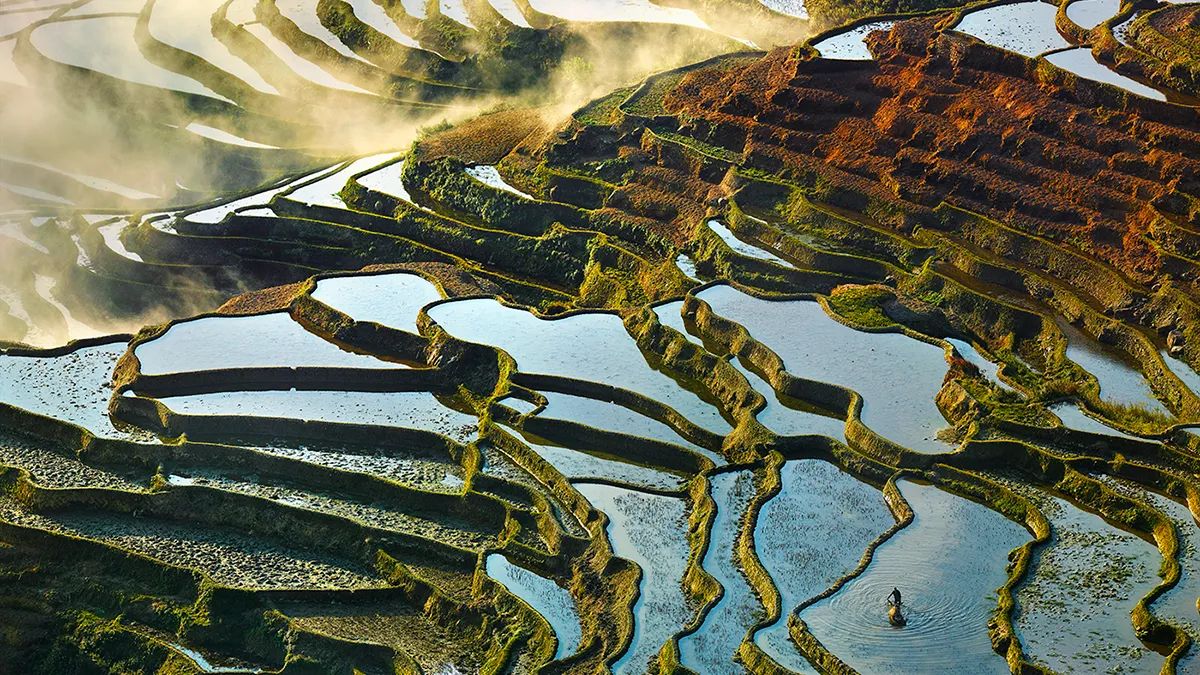
\includegraphics[width=\textwidth]{rice_paddy}

	\textit{thousand year old rice paddy}

\end{frame}


\begin{frame}{Terraforming Vim}

	\begin{block}{Technical Terraforming}

		\vspace{0.5em}

		Making nvim more hospitable for developers

		\vspace{0.5em}

	\end{block}

	\rule{\textwidth}{0.1em}

	\begin{itemize}

		\begin{multicols}{2}

			\item lua

			\item vim.api.nvim\_*

			\item API clients

			\item tree-sitter

			\item libuv

			\item extmarks

			\item virtual text

			\item remote UI

		\end{multicols}

	\end{itemize}

	... and more

\end{frame}


\begin{frame}{Yes We Can}

	Short detour

	\rule{\textwidth}{0.1em}

	Lua is powerful

	You can write \textit{async await} as a \textbf{library}, (first class coroutines)

	https://github.com/ms-jpq/lua-async-await

	\hspace{0.1em}

	\textit{(Like Clojure core.async)}

\end{frame}


\begin{frame}[standout]

	Ossification of Ecosystem

\end{frame}


\begin{frame}{Vim "philosophy"}

	\begin{itemize}

		\begin{multicols}{2}

			\item unix-y

			\item ad hoc

			\item macro driven

			\item minimalist

			\item extensible

			\item composible

			\item conservative

			\item worse is better

		\end{multicols}

	\end{itemize}

\end{frame}


\begin{frame}{Weight of History}

	\begin{itemize}

		\begin{multicols}{2}

			\item slowiness

			\item jankiness

			\item ossification

			\item interlocking

			\item beginner hostile

			\item dx hostile

		\end{multicols}

	\end{itemize}

\end{frame}


\begin{frame}[standout]

	Ossification of Habits

\end{frame}


\begin{frame}{Users, Users, Users}

	\begin{block}{Cultural Terraforming}

		\vspace{0.5em}

		Realizing the benefits of change is a two way street

		Need user buy in

		\vspace{0.5em}

	\end{block}

\end{frame}


\begin{frame}{Tolerance for Heresy}

	Beyond just the API, but also the \textbf{culture too}

	\rule{\textwidth}{0.1em}

	\textbf{Wait, you can do that??}

	\begin{enumerate}

		\item nvim = Browser for TUI

		\item buffers = render targets

		\item architecture <- systematic, data driven

		\item "AOT compiled, statically linked"

		\item Well defined protocols

	\end{enumerate}

\end{frame}


\begin{frame}{High Aspirations}

	\textbf{Nvim wants to be a platform}

	\textit{Browser for the TUI}

	\rule{\textwidth}{0.1em}

	\hspace{0.1em}

	\begin{block}{Official API Clients}

		\begin{itemize}

			\begin{multicols}{2}

				\item c\#

				\item go

				\item node

				\item python

				\item ruby

			\end{multicols}

		\end{itemize}

	\end{block}

	And tons and tons of unofficial ones..

\end{frame}


\begin{frame}{We Are Not There Yet}

	Lots of UIs, not many client-server plugins

	\textbf{Unrealized Potentials}

	\rule{\textwidth}{0.1em}

	People want a faster horse.

	Faster horse not good enough to break habits.

	\hspace{0.1em}

	Need \textbf{\textit{significant value proposition}}.

\end{frame}


\begin{frame}[standout]

	Broken eggs, no omelettes?

	Time to write nice things.

\end{frame}


\begin{frame}{Do Different}

	\begin{block}{Kitchen sink}

		\vspace{0.5em}

		Do one \st{thing} \textbf{domain} and do it well.

		\vspace{0.5em}

		\textbf{Don't expose implementations}

	\end{block}

	\rule{\textwidth}{0.1em}

	\textit{Extensibility still possible}

\end{frame}


\begin{frame}{AOT Static Linking}

	\hspace{0.1em}

	Dual Approach:

	\begin{enumerate}

		\item \st{Web} Vim Scrapping

		\item Write it yourself (but do it good)

	\end{enumerate}

\end{frame}


\begin{frame}{Ossification -> Unofficial API}

	"Zero runtime cost" -- \st{rust} JSON

	\begin{enumerate}

		\item Compile \text{existing plugins} for artifacts

		\item Dump them into a static file

	\end{enumerate}

	\rule{\textwidth}{0.1em}

	\begin{itemize}

		\item CHADTree

		      \begin{itemize}

			      \item 3 icon themes

			      \item 9 colour themes

			      \item 700+ language colours

		      \end{itemize}

		\item COQ.nvim

		      \begin{itemize}

			      \item 13,000+ snippets

			      \item \textbf{zero runtime parse errors}

		      \end{itemize}

	\end{itemize}

\end{frame}


\begin{frame}{\$LS\_COLORS}

	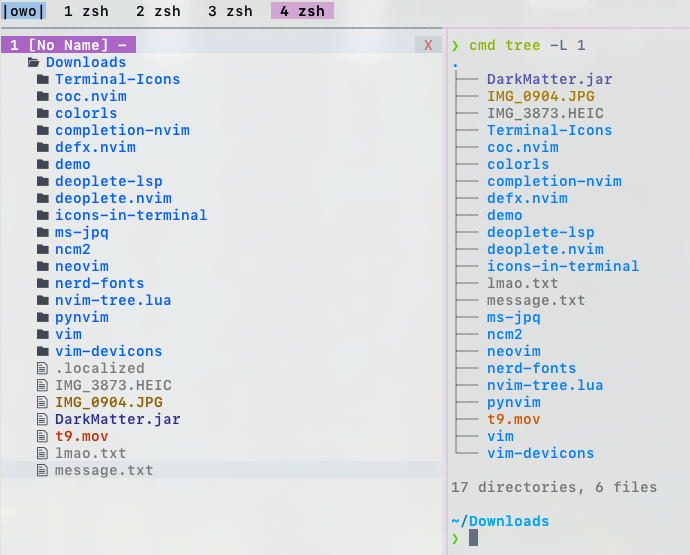
\includegraphics[width=\textwidth,height=20em]{chadtree_ls}

\end{frame}


\begin{frame}{Python Faster than LUA?}

	\begin{block}{Observations}

		\begin{enumerate}

			\item File system walking is very fast

			\item Rendering is slow

			\item Decoration plugins cause dramatic slowdowns

		\end{enumerate}

	\end{block}

	\hspace{0.1em}

	\begin{block}{Solution}

		\begin{itemize}

			\item Pull in decorations

			\item Minimize rendering

		\end{itemize}

	\end{block}

\end{frame}


\begin{frame}{React!}

	I wrote a \textit{70 line} React before, it's not hard:

	https://github.com/ms-jpq/noact

	\rule{\textwidth}{0.1em}

	Virtual rendering target

	\begin{enumerate}

		\item Compute desired state

		\item Compute linewise hash of desired state

	\end{enumerate}

	Actual rendering target (apply state to buffers)

	\begin{enumerate}

		\item Fetch hash -> compute minimal diff

		\item Apply patch onto buffers, store new hash

	\end{enumerate}

\end{frame}


\begin{frame}{CHADTree: Other Features}

	https://github.com/ms-jpq/chadtree

	\rule{\textwidth}{0.1em}

	\begin{itemize}

		\begin{multicols}{2}

			\item visual multi selection

			\item persistent selection across copy / move

			\item quickfix highlight

			\item glob filtering

			\item trash bin

			\item open with sys

			\item ls -l

			\item follow mode

			\item version control status

			\item \$LS\_COLOUR theming

			\item icons out of box

			\item github derived language colouring

			\item session support

			\item typed config parser

		\end{multicols}

	\end{itemize}

\end{frame}


\begin{frame}{Config Parser}

	Type checker for plugin configuration

	\rule{\textwidth}{0.1em}

	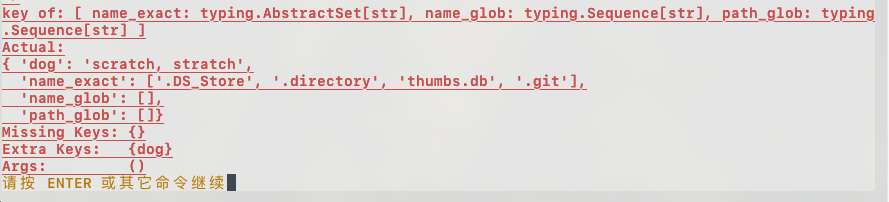
\includegraphics[width=\textwidth]{conf_parser}

	Added extra "dog" key

\end{frame}


\begin{frame}{COQ.nvim}

	Fast AF auto completion, backed by \textit{SQLite}

	https://github.com/ms-jpq/coq\_nvim

	\rule{\textwidth}{0.1em}

	Can't just AOT everything

	\textbf{Has to be extensible}

\end{frame}


\begin{frame}{Ossification Kills}

	Need to support third party plugins, but...

	Notice a pattern here:

	\begin{itemize}

		\item nvim-completion-manager -> ncm2

		\item neocomplete.vim -> deoplete.nvim -> ddc.vim

		\item nvim-compe -> nvim-cmp

		\item completion-nvim -> \st{still ok!} \textit{archived}

	\end{itemize}

	Too big to rewrite:

	\begin{itemize}

		\item YouCompleteMe

		\item coc.nvim

	\end{itemize}

\end{frame}


\begin{frame}[standout]

	Move Fast Without Breaking Things

\end{frame}


\begin{frame}{The Protocols of Nvim}

	Protocols are \textbf{meant to be ossified}

	Implementations are not

	\rule{\textwidth}{0.1em}

	Some protocols are \textit{accidental} or \textit{emergent}

	\begin{itemize}

		\item vim.bo.omnifunc

		\item :h complete-items

		\item \textbf{LSP}

	\end{itemize}

\end{frame}


\begin{frame}{Social Distancing}

	No Importable Code

	\rule{\textwidth}{0.1em}

	Third party code \textbf{CAN NOT} call into coq.nvim

	They register callbacks at well known locations (Vim Tradition)

	Callbacks communicate via \textbf{Existing} Protocols

	\rule{\textwidth}{0.1em}

	https://github.com/ms-jpq/coq.thirdparty

\end{frame}


\begin{frame}{PaaS}

	What is the platform

	\rule{\textwidth}{0.1em}

	\begin{itemize}

		\item Your app is not the \textbf{platform}

		\item Nvim is the \textbf{platform}

		\item Ecosystem is the \textbf{platform}

	\end{itemize}

\end{frame}


\begin{frame}[standout]

	Worse is Not Always Better

\end{frame}


\begin{frame}{When to Break Traditions}

	Worse is better for \textbf{software} not \textbf{wetware}

	\rule{\textwidth}{0.1em}

	\begin{itemize}

		\item Computers fast

		\item Meatbags slow

	\end{itemize}

	\rule{\textwidth}{0.1em}

	\st{Implementations Simplicity} Humans are not computers

\end{frame}


\begin{frame}{Humans Suck}

	Designing for meatbags.

	\rule{\textwidth}{0.1em}

	\begin{block}{Observations}

		\begin{itemize}

			\item Computers are \textit{fast}, humans are \textit{slow}

			\item Humans can't typo good

			\item Humans have low working memory

		\end{itemize}

	\end{block}

	Worth breaking traditions...

\end{frame}


\begin{frame}{Speed of Humans}

	Optimization problem:

	\rule{\textwidth}{0.1em}

	\begin{itemize}

		\item Humans are slow readers \& bad typers

		\item Relevant results paramount\footnote{Larry Page $\approx$ 120B}

		\item Must tolerate errors

		\item Trade machine time for human time.

	\end{itemize}

\end{frame}


\begin{frame}{Data Driven Completion Ranking}

	Robust against 2 character typos\footnote{except in first 2 characters}

	\rule{\textwidth}{0.1em}

	Link to 2 stage algorithm

	https://github.com/ms-jpq/coq\_nvim/blob/coq/docs/FUZZY.md

	\rule{\textwidth}{0.1em}

	Borrow ideas from ML's data processing

	Weights, normalization \& sigmoid func adjust for user inputs

\end{frame}


\begin{frame}{Provide as Much Info as Possible}

	CTags

	
\includegraphics[width=\textwidth]{info_ctags}

	Paths

	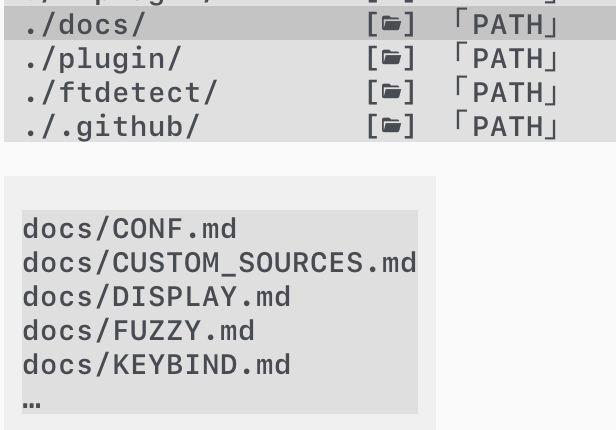
\includegraphics[keepaspectratio,width=\textwidth,height=9em]{info_paths}

\end{frame}


\begin{frame}{COQ::REPL}

	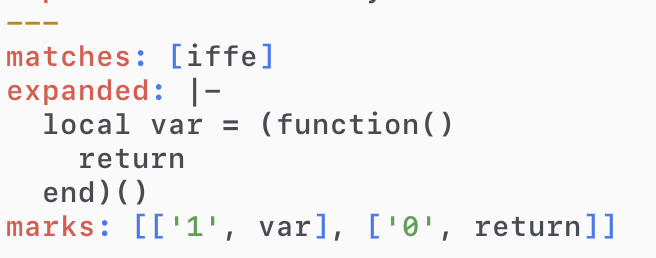
\includegraphics[width=\textwidth]{repl_succ}

	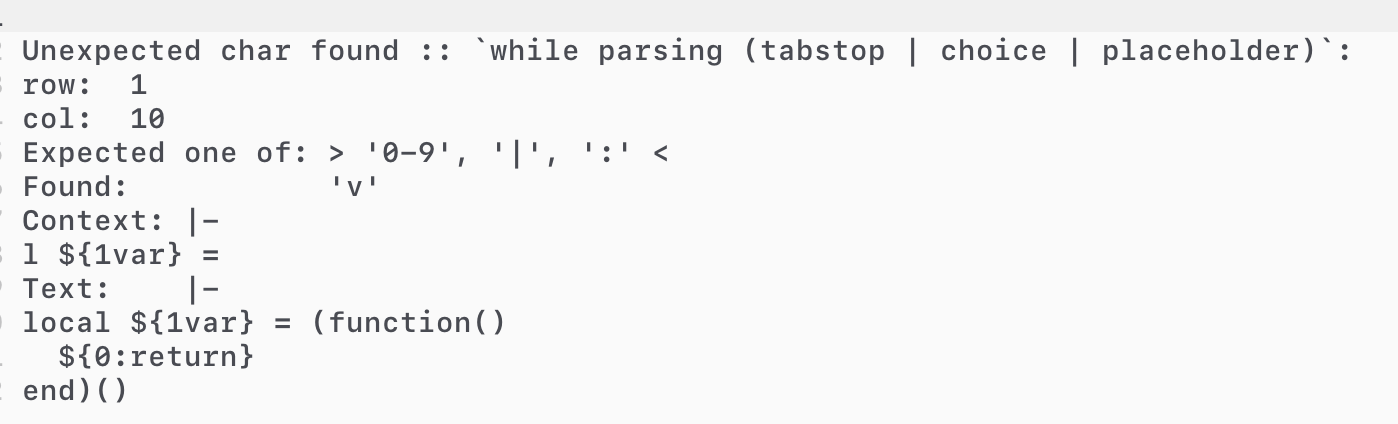
\includegraphics[width=\textwidth]{repl_fail}

\end{frame}


\begin{frame}{COQ::Stats}

	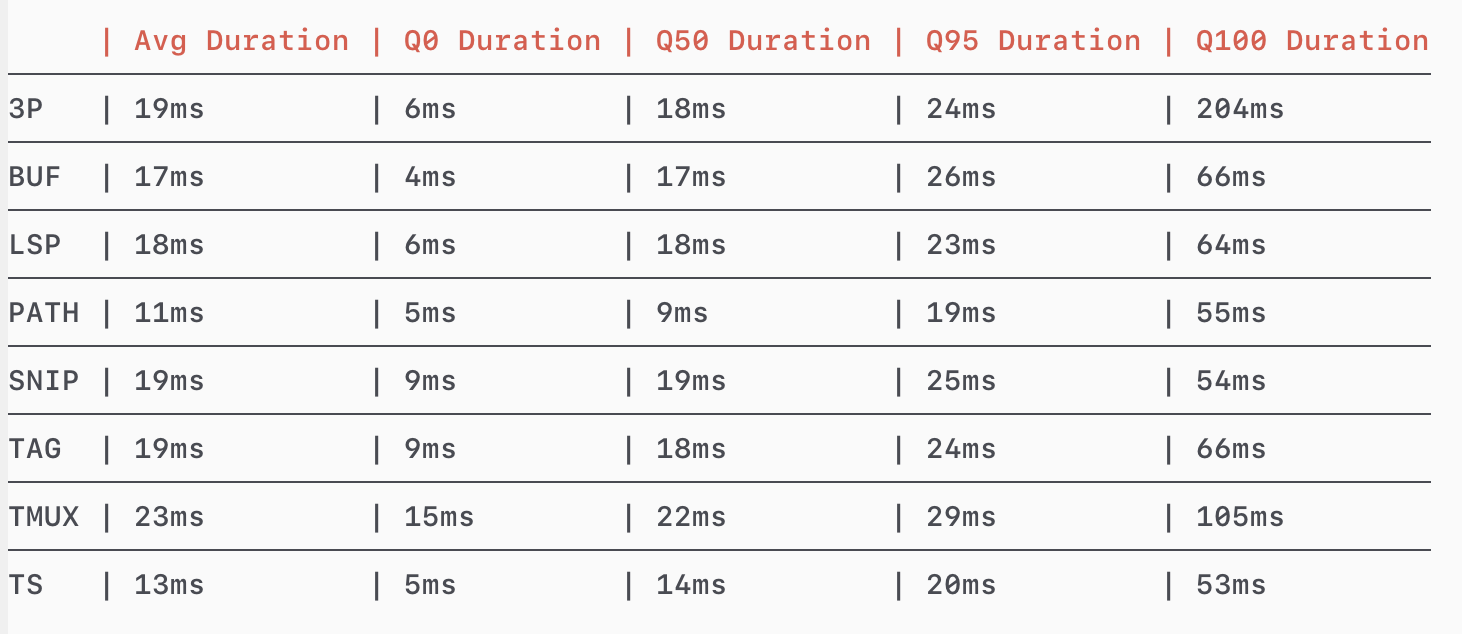
\includegraphics[width=\textwidth]{stats}

\end{frame}


\begin{frame}{Scheduler}

	\begin{itemize}

		\item \textbf{What} is a unit of work?

		\item \textbf{When} is work performed

		\item \textbf{If} work is performed

	\end{itemize}

\end{frame}


\begin{frame}{Out of Time}

	They all need their own slides

	\begin{itemize}

		\item Concurrency is not parallelism

		\item Python GIL

		\item Manual SQLite preemption

		\item Tradeing \textit{throughput} for \textit{latency}

		\item Ubiquitous lazy computation

		\item Coroutine scheduling

		\item Cancel culture

		\item Flow control

		\item Background caching

		\item Soft deadlines

	\end{itemize}

\end{frame}


\begin{frame}{Still AOT}

	The most completion sources out of the box

	\begin{itemize}

		\item LSP - multi-server, clientside caching, snippet support

		\item Snippets - over 13000 built-in, live repl, custom snips

		\item Treesitter - partial parsing, disable disable if slow, LSP like context

		\item CTags - LSP like metadata, background compilation, sqlite instead of nvim's blocking built-in

		\item Paths - previews contents, variable expansion

		\item Buffers - real time

		\item Tmux

		\item Tabnine - auto download

	\end{itemize}

\end{frame}


\begin{frame}{Even More LUA Sources}

	\begin{itemize}

		\item Shell REPL

		\item Nvim LUA API

		\item Scientific calculator

		\item Commented banner

	\end{itemize}

\end{frame}


\begin{frame}{Benchmarks}

	https://github.com/ms-jpq/vim.bench

	\rule{\textwidth}{0.1em}

	Reproducible Docker based tmux typist

	Kernel density estimates

\end{frame}


\begin{frame}{Tying the Knot}

	\begin{centering}

		{\Large Technical Innovation $\cup$ Cultural Innovation}

		\rule{\textwidth}{0.1em}

		{\LARGE Nice things}

	\end{centering}

\end{frame}


\begin{frame}[standout]

	Q \& A

\end{frame}


\end{document}
